\documentclass[11pt]{article}

\usepackage{custom}
\newcolumntype{R}[1]{>{\raggedleft\arraybackslash}m{#1}}

\title{605.744: Information Retrieval \\ Emotion Extraction From Lyrics}
\author{Sabbir Ahmed}
\date{\today}

\begin{document}
\maketitle
\tableofcontents
\clearpage
\newpage

\begin{abstract}
  \noindent Mood classification in music has become more prevalent with the growing streaming industry. Categorizing songs based on the perceived emotions allow music streaming services to improve their recommendation systems and automatic playlist generation. Services such as Spotify use audio features such as duration, energy, tempo, etc. and other combinations of audio features such as danceability and instrumentalness to group similar tracks. These classifications focus solely on the audio production of the songs while ignoring the lyrical content. Emotion extraction from text can be a difficult task, due to the subjectivity in quantifying or discretely categorizing emotions. In this project, 2 of the popular models of emotions, the Plutchik's Wheel and the VAD model, have been used to attempt emotion extraction.
\end{abstract}

\section{Introduction}
This paper discusses the methods used to

\section{Background}

\subsection{Natural Language Processing on Lyrics}

Natural language processing on English song lyrics assume additional restrictions. There are no standards set for preprocessing lyrics, but the following lists the exceptions address for this project:
\begin{itemize}
  \item Songs may be entirely composed of stopwords.
  \item Repetition is considered significant.
  \item Lyrics may contain songwriting directions, such as "[gang vocals]", "[instrumental]", "[hook]", "[Speaker A]", etc.
  \item Lyrics may contain adlibs. For this project, adlibs are not considered part of the dictionary.
\end{itemize}

\subsection{Sentiment Analysis}

Sentiment scores are evaluated as the ratios of weights of the relatively positive and negative terms in a document. Context is typically emphasized to increase the accuracy of the perceived sentiment. This is achieved by using long n-grams. This project tokenizes the documents as 1-grams, and therefore loses contexts. The sentiment scores are instead evaluated as the ratio of the positive terms ($p$) and negative terms ($n$) over the total number of terms. Terms are labeled positive or negative if they are found in their corresponding datasets.

\begin{equation}
  S = \frac{|p| - |n|}{N}
\end{equation}

If a document contains more negative terms, then the sentiment score will naturally be negative as well, and vice versa for a positive score.

\subsection{Emotion Classification}

The field of emotion classification is highly subjective. It is often difficult to quantify with absolute values or discretely classify emotions. There have been several psychological models developed over the decades. This project utilizes 2 of the popular models, the Plutchik's Wheel of Emotions and the VAD Emotional State Model.

\subsubsection{Plutchik's Wheel of Emotions Model}

Psychologist Robert Plutchik proposed a model composed of eight primary emotions: anger, fear, sadness, disgust, surprise, anticipation, trust, and joy \cite{wheel}. The model, pictured in Figure \ref{fig:wheel}, consists of several concentric circles, with the outer circles being combinations of emotions from the inner circles.

\begin{figure}[!ht]
  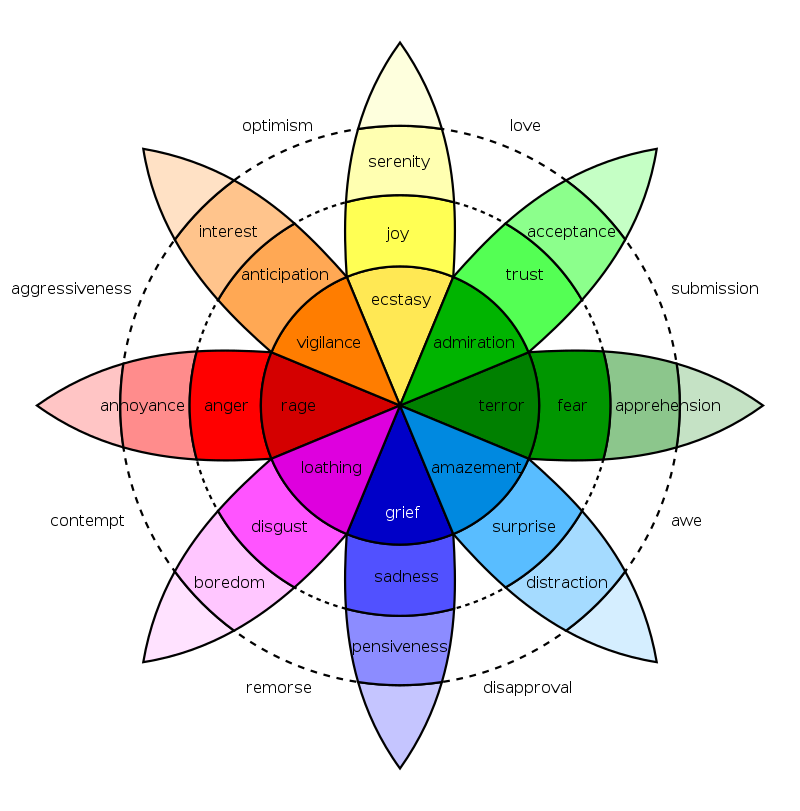
\includegraphics[scale=0.4]{../statics/wheel.png}
  \centering
  \caption{Plutchik's Wheel of Emotions Model}
  \label{fig:wheel}
\end{figure}

% Several categories described by the model do not translate well over text. For example, a human reviewer may infer emotions such as \textit{disgust} and \textit{anger} from the document "Good God, the venerable saint was romancing the scientist's bride!". The prevalent emotions extracted from the document using the emotion intensities are \textit{trust} and \textit{anticipation}.

Several categories described by the model do not translate well over text. For example, a human reviewer may find it difficult to extract emotions of \textit{trust} or \textit{anticipation} from a document without explicit usages of synonyms of such emotions.

\subsubsection{VAD Emotional State Model}

The VAD (Valence-Arousal-Dominance) Emotional State Model was proposed by psychologist Albert Mehrabian. The model plots emotional states across these 3 dimensions of emotion. Valence measures how pleasant or unpleasant an emotion is, arousal determines the energy of the emotion, and dominance refers to the sense of control over the particular emotion. The model, pictured in \ref{fig:vad}, implies a more granular approach to categorizing emotions.

\begin{figure}[!ht]
  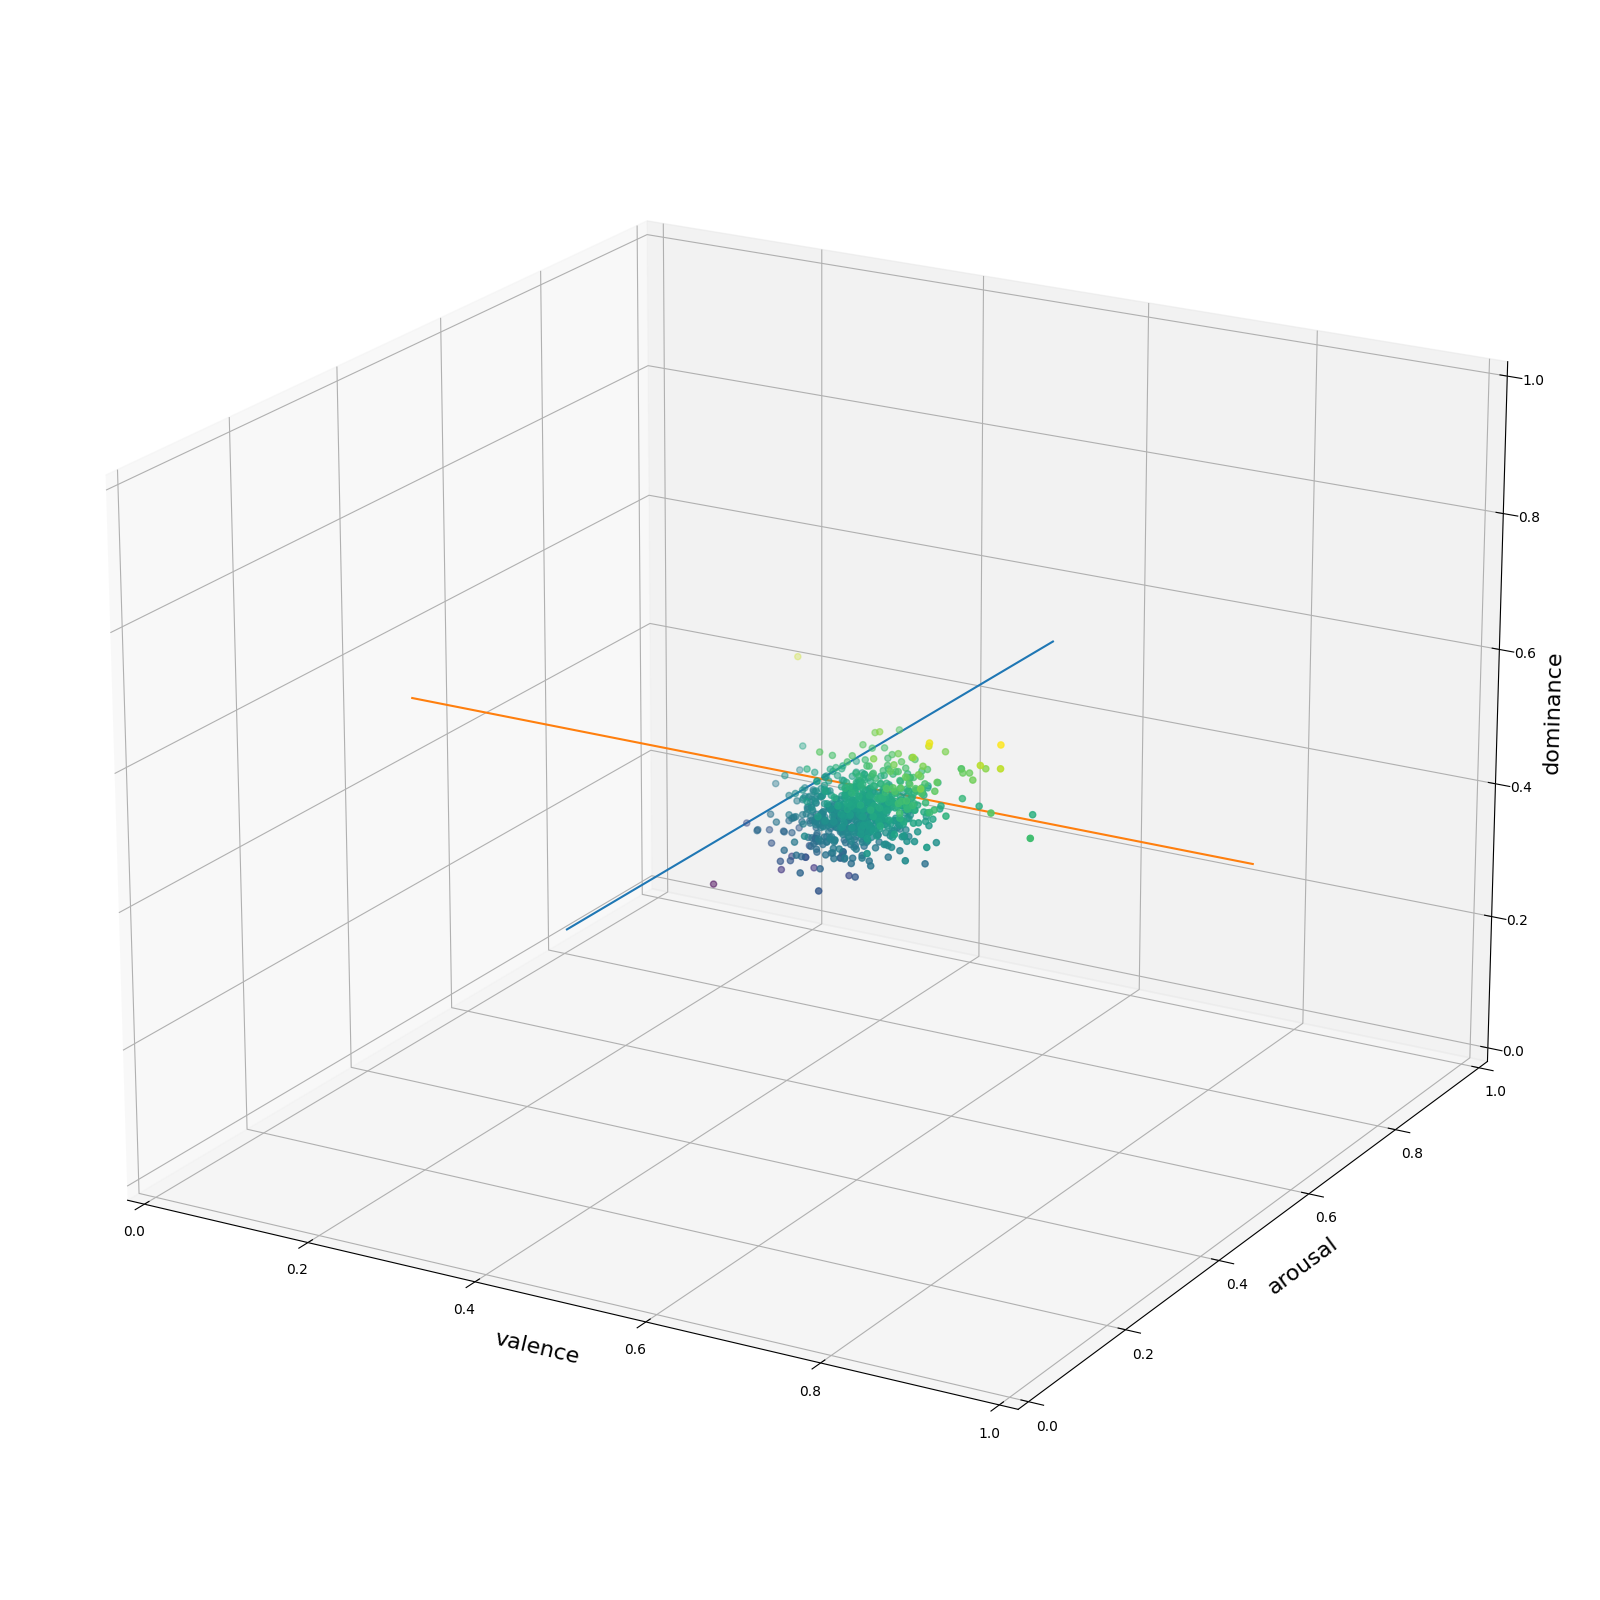
\includegraphics[scale=0.35]{../statics/vad.png}
  \centering
  \caption{VAD Emotional State Model}
  \label{fig:vad}
\end{figure}

The third dimension of the model can be disregarded to describe the more popular Valence-Arousal Emotional State Model (also known as the Circumplex Model), developed by psychologist James A. Russell. The two dimensions of this model allows for emotions to be categorized into quadrants which are sufficient in determining the general sentiment of the emotion. The four quadrants can be labeled as:
\begin{itemize}
  \item \textbf{Quadrant I}: High-arousal/positive-valence, "joy"
  \item \textbf{Quadrant II}: High-arousal/negative-valence, "anger"
  \item \textbf{Quadrant III}: Low-arousal/negative-valence, "sadness"
  \item \textbf{Quadrant IV}: Low-arousal/positive-valence, "calm"
\end{itemize}

\begin{figure}[!ht]
  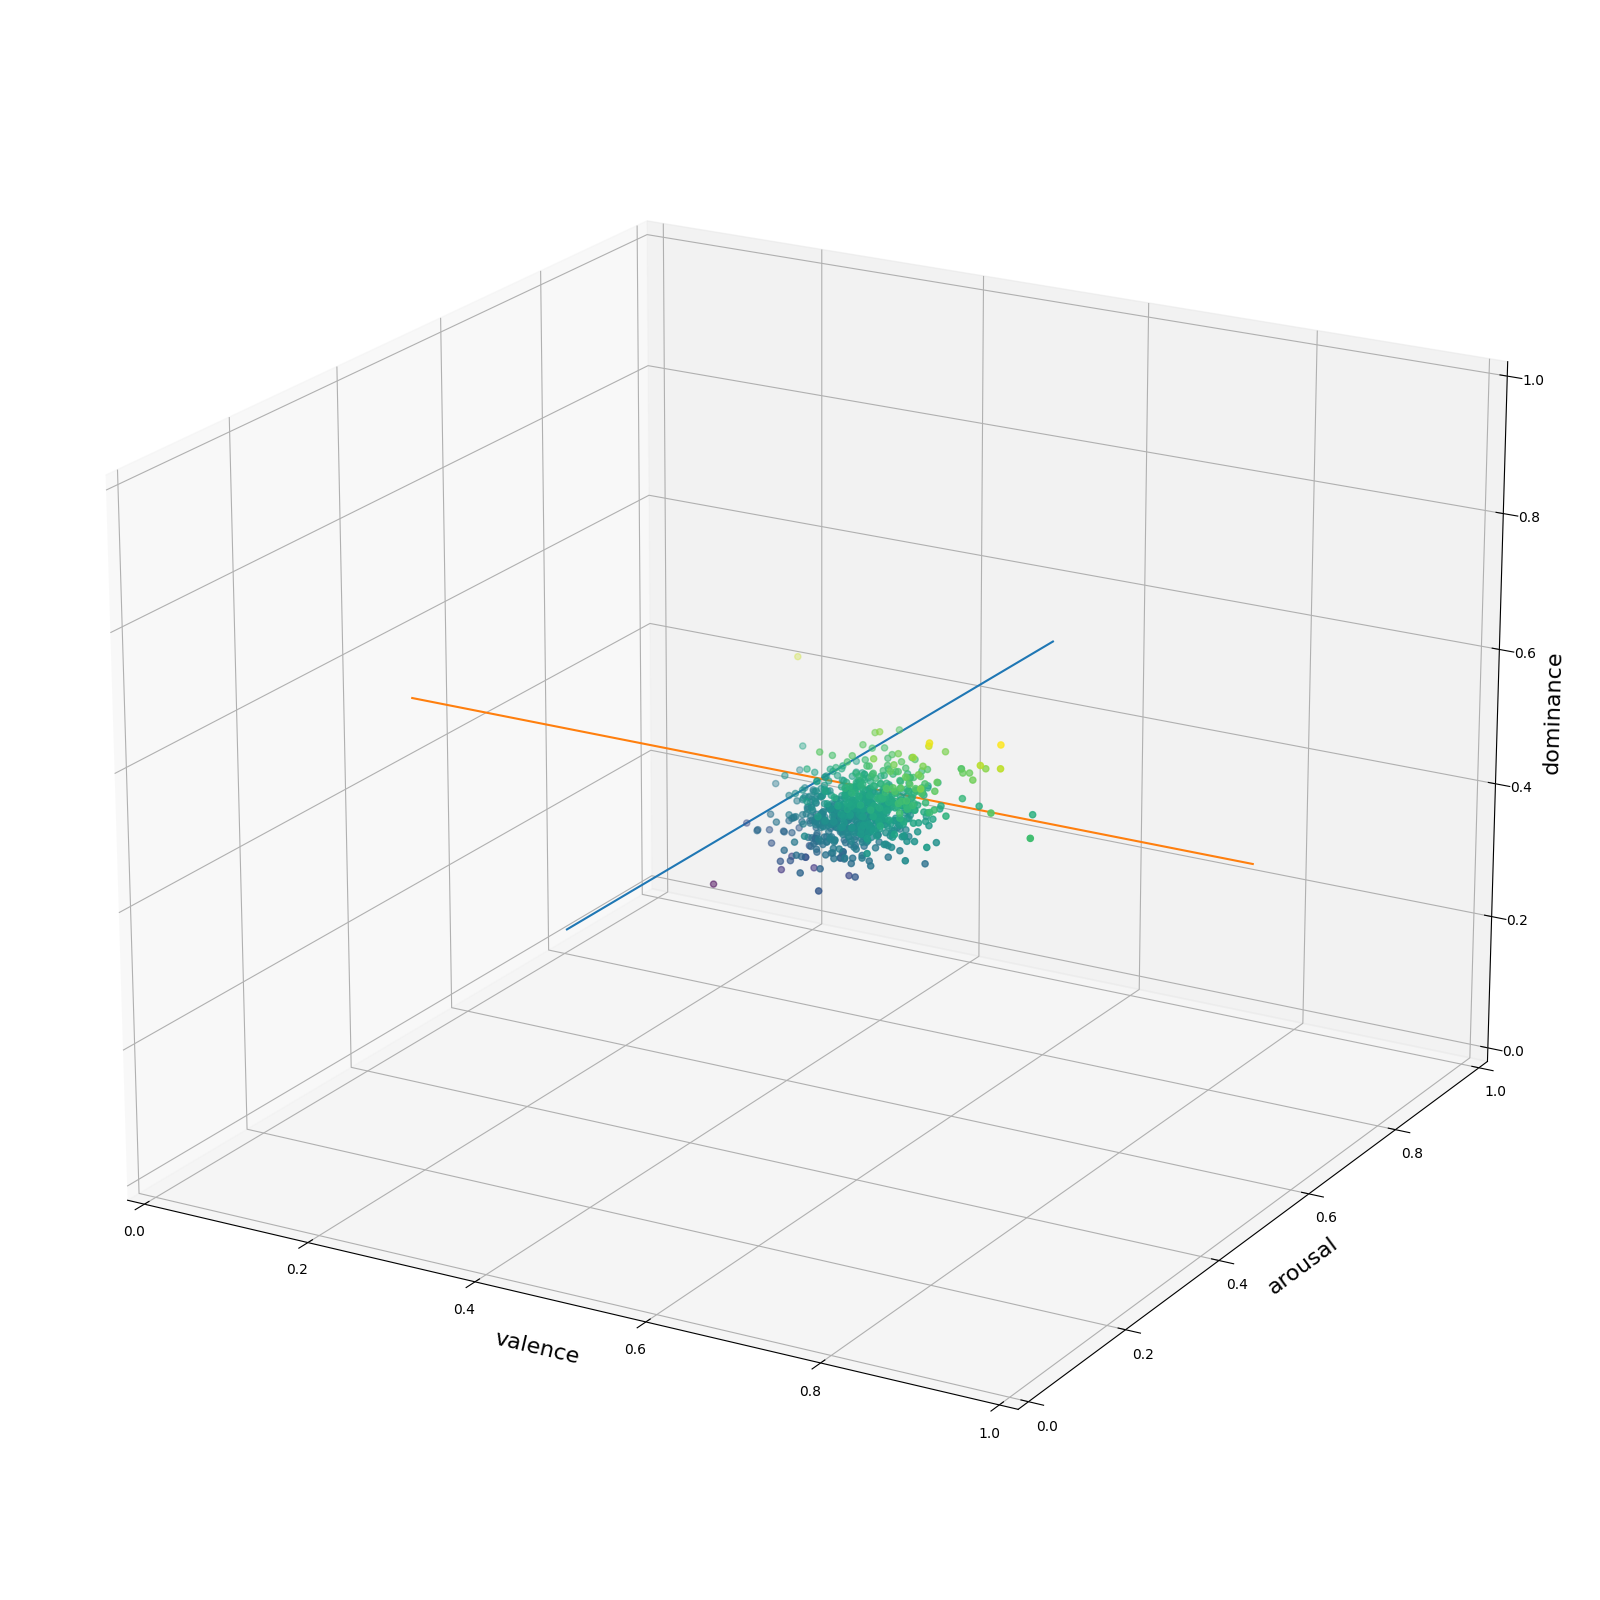
\includegraphics[scale=0.35]{../statics/vad.png}
  \centering
  \caption{VAD Emotional State Model}
  \label{fig:va}
\end{figure}

\section{Source Datasets}

The datasets for this project were obtained from various sources.

\subsection{Playlist Datasets}

Playlist datasets were obtained from Spotify via their web application programming interface (API) \cite{spotify}. Top playlists curated by the Spotify staff were randomly selected, and the API was used to gather playlist names, lists of tracks, and the apparent targeted moods.

\subsection{Lyrics}

The lyrics of all of the tracks from the playlist datasets were obtained via scraping from various web sources. In total, 748 documents were obtained for analysis.

\subsection{NRC Emotion Lexicons}

The word associations, emotion intensities and the VAD lexicons for the emotion models were obtained from the National Research Council Canada \cite{LREC18-AIL,Mohammad13,vad-acl2018}. The dictionaries for the positive and negative terms required to compute the sentiment scores were also extracted from these datasets.

\section{Scores}

The scores generated are based on sums of the emotion intensities and frequencies of word associations.

\subsection{Emotion Intensity}

Emotion intensity scores are generated for the 8 emotions identified by the Plutchik's Wheel Model. The scores are simply the sums of the corresponding emotion intensity values present in the NRC datasets. To normalize the intensity scores, each of the 8 emotions also have their corresponding intensity ratio scores, which are calculated by computing the ratio of the emotion intensities over the total sum of intensities. Equation \ref{equ:emo_ratio} defines the ratio for all emotions $e$ in the 8 emotions identified by the Plutchik's Wheel Model, $E$.

\begin{equation} \label{equ:emo_ratio}
  e_{ratio} = \frac{\sum_{i=0}e_i}{\sum_{e \in E}\sum_{i=0}e_i}
\end{equation}

\subsection{VAD Scores}

Similar to the emotion intensity scores, the valence, arousal and dominance scores were evaluated by summing their intensities and averaging them over the number of terms identified in the word associations. Since every term in the dataset are associated with a 3-tuple of valence, arousal and dominance values, their sums are averaged by the same value. Equation \ref{equ:vad} defines the ratios.

\begin{equation} \label{equ:vad}
  v = \frac{\sum_{i=0}^{N}v_i}{N}, a = \frac{\sum_{i=0}^{N}a_i}{N}, d = \frac{\sum_{i=0}^{N}d_i}{N}
\end{equation}

\section{Analysis}

\begin{simptable}
  {No transform}
  {scores}
  {|c|c|c||c|c||c|c|}
  \textbf{Emotion} & \textbf{mean} & \textbf{median} & \textbf{mean} & \textbf{median} & \textbf{mean} & \textbf{median}\\
  \hline
  anticipation &  1.730709 &  1.5940 &  3.719128 &  2.8350 &  1.730709 &  1.5940 \\
  \hline
  disgust      &  1.069293 &  0.7200 &  2.601124 &  1.1640 &  1.069293 &  0.7200 \\
  \hline
  anger        &  1.648021 &  1.2190 &  3.986169 &  1.8750 &  1.648021 &  1.2190 \\
  \hline
  trust        &  2.476561 &  2.1790 &  6.776188 &  4.9530 &  2.476284 &  2.1790 \\
  \hline
  sadness      &  1.790973 &  1.5090 &  3.842015 &  2.6960 &  1.701007 &  1.4210 \\
  \hline
  joy          &  2.392433 &  2.2070 &  6.319867 &  4.4240 &  2.392433 &  2.2070 \\
  \hline
  fear         &  1.888261 &  1.5315 &  3.869922 &  2.4785 &  1.888261 &  1.5315 \\
  \hline
  surprise     &  0.851107 &  0.7420 &  1.840037 &  1.0710 &  0.851107 &  0.7420 \\
  \hline
\end{simptable}

\begin{simptable}
  {ratio}
  {scores}
  {|c|c|c|c|}
  \textbf{Emotion} & \textbf{mean} & \textbf{median} & \textbf{max} \\
  \hline
  joy\_ratio          &  0.216300 &  0.218978&  0.668980 \\
  \hline
  trust\_ratio        &  0.186233 &  0.187097&  0.638021 \\
  \hline
  sadness\_ratio      &  0.121942 &  0.114320&  0.457091 \\
  \hline
  surprise\_ratio     &  0.057528 &  0.052510&  0.407974 \\
  \hline
  anticipation\_ratio &  0.138459 &  0.138032&  0.456406 \\
  \hline
  anger\_ratio        &  0.101198 &  0.090794&  0.694792 \\
  \hline
  disgust\_ratio      &  0.065279 &  0.057565&  0.316643 \\
  \hline
  fear\_ratio         &  0.113061 &  0.106388&  0.409779 \\
  \hline
\end{simptable}

% \section{Technical Background}
% All of the source code is in Python 3.10. The program is split into several modules and follows an object oriented structure.

\subsection{Emotion Playlist}

\begin{equation}
  acc = \frac{\sum_{p \in E^{+}}\frac{\sum_{i}[p_i > 0]}{|p|} + \sum_{n \in E^{-}}\frac{\sum_{i}[n_i < 0]}{|n|}}{|E|}
\end{equation}

% Original count: 748


\begin{simptable}
  {ratio}
  {scores}
  {|c|c|c|}
  \textbf{Metric} & \textbf{Tracks Categorized} & \textbf{Accuracy} \\
  \hline
  25\%  & 747 & 0.544 \\
  \hline
  50\%  & 747 & 0.643 \\
  \hline
  75\%  & 730 & 0.747 \\
  \hline
  mean  & 747 & 0.673 \\
  \hline
\end{simptable}

\begin{simptable}
  {ratio}
  {scores}
  {|c|c|c|}
  \textbf{Metric} & \textbf{Tracks Categorized} & \textbf{Accuracy} \\
  \hline
  25\%  & 626 & 0.572 \\
  \hline
  50\%  & 626 & 0.719 \\
  \hline
  75\%  & 603 & 0.820 \\
  \hline
  mean  & 626 & 0.713 \\
  \hline
\end{simptable}


\begin{simptable}
  {ratio}
  {scores}
  {|c|c|}
  \textbf{wheel\_playlist} & \textbf{count} \\
  \hline
  fear &  490 \\
  \hline
  disgust &  474 \\
  \hline
  anger &  470 \\
  \hline
  sadness &  470 \\
  \hline
  anticipation &  469 \\
  \hline
  trust &  461 \\
  \hline
  surprise &  458 \\
  \hline
  joy &  444 \\
  \hline
\end{simptable}

\addcontentsline{toc}{section}{References}
\bibliographystyle{ieeetr}
\bibliography{refs}

\end{document}
